\documentclass{beamer}
\usepackage[utf8]{inputenc}
\usepackage[english]{babel}
\usepackage{verbatim}
\usepackage{listings}
\usepackage{graphicx}
\usepackage{amsmath}
\usepackage{array}
\usepackage{xcolor}
\usepackage{pgf}
\usepackage{tikz}
\usetikzlibrary{arrows,calc,intersections,through,
    decorations.pathmorphing,backgrounds,positioning,fit}
\usepackage[T1]{fontenc}
\usepackage{minted}
\usepackage{ulem}
\usetheme{gapz}

\title{Ansible on arch 101}
\author{Julien Girardin}

\date{\today}

\begin{document}

\maketitle{}

\begin{frame}
    \frametitle{Why Ansible?}
    \begin{tabular}{>{\centering}m{2cm}|>{\centering}m{2.5cm}|>{\centering}m{2.5cm}|>{\centering}m{2.45cm}|@{}m{0pt}@{}}
        \cline{2-4}
                                      & Puppet            & Chef              & Ansible      &\\[10pt] \hline
    \multicolumn{1}{|c|}{Architecture}& Server \& Agent   & Server \& Agent   & Workstation  &\\[10pt] \hline
    \multicolumn{1}{|c|}{Security}    & Certificates(PKI) & Certificates(PKI) & SSH          &\\[10pt] \hline
    \multicolumn{1}{|c|}{Language}    & DSL               & Ruby              & DSL          &\\[10pt]\hline
    \multicolumn{1}{|c|}{Extension}   & Ruby              & Ruby              & Python       &\\[10pt]\hline
    \multicolumn{1}{|c|}{Push/Pull}   & Pull              & Pull              & Push         &\\[10pt] \hline

    \end{tabular}
\end{frame}

\begin{frame}[fragile]
\frametitle{How it works}
\begin{figure}[!h]
    \centering{
    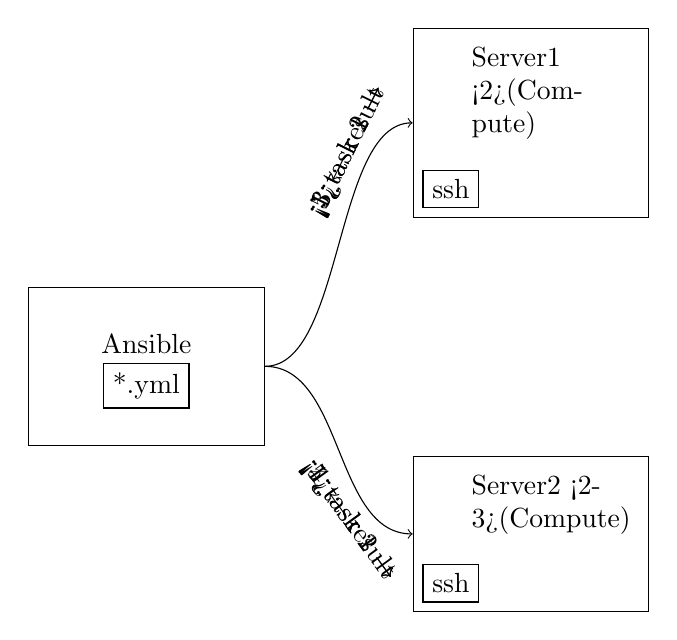
\begin{tikzpicture}
        %\node[shape=rectangle, draw,]              (yml1)      {yml};
        %\node[shape=rectangle, draw, draw opacity=1,
        %   opacity=1,fill=none, fill opacity=1,
        %   xshift=-0.1cm, yshift=0.1cm]            (yml2)      {yml};
        \node[shape=rectangle, draw,
                xshift=-0.2cm, yshift=0.2cm]        (yml3)      {*.yml};
        \node[above = of yml3, yshift=-1cm]         (a)         {Ansible};
        \node[shape=rectangle, draw,
            minimum width=3cm,
            minimum height=2cm,
            fit=(a) (yml3)]                         (ansible)   {};

        \node[above right= of ansible,
                xshift = 1.5cm, yshift = 0.75cm,
                text width=2cm ]                    (s1)
                {Server1 {\visible<2>{(Compute)}}};
        \node[shape=rectangle, draw,
             above right= of ansible,
                xshift = 1cm]                           (ssh1)      {ssh};
        \node[shape=rectangle, draw, fit=(s1) (ssh1)]   (server1)   {};

        \node[below right= of ansible,
                xshift = 1.5cm, yshift = 0.75cm,
                text width=2cm ]    (s2)
                {Server2 {\visible<2-3>{(Compute)}}};
        \node[shape=rectangle, draw,
            below right= of ansible,
            xshift=1cm, yshift=-0.5cm]                  (ssh2)      {ssh};
        \node[shape=rectangle, draw, fit=(s2) (ssh2)]   (server2)   {};

        \draw[->]
            (ansible.east) .. controls +(right:1cm) and +(left:1cm) ..
            (server1.west)
            node[near end,sloped, above]
                {{\visible<1>{task 1 $\rightarrow$}}}
            node[near end,sloped, above]
                {{\visible<3>{$\leftarrow$ result}}}
            node[near end,sloped, above]
                {{\visible<5>{task 2 $\rightarrow$}}}
        ;
        \draw[->]
            (ansible.east) .. controls +(right:1cm) and +(left:1cm) ..
                (server2.west)
            node[near end,sloped, below]
                {{\visible<1>{task 1 $\rightarrow$}}}
            node[near end,sloped, below]
                {{\visible<4>{$\leftarrow$ result}}}
            node[near end,sloped, below]
                {{\visible<5>{task 2 $\rightarrow$}}}
        ;
    \end{tikzpicture} }
\end{figure}
\end{frame}


\begin{frame}[fragile]
\frametitle{For archlinux ?}

    \begin{block}{/etc/ansible/hosts or -i filename}
        \begin{minted}{text}
[webservers]
foo1.arkena.test ansible_python_interpreter=python2
foo2.arkena.test # not an archlinux based server

[dbservers]
bar.arkena.test  ansible_python_interpreter=python2
        \end{minted}
    \end{block}
AND
    \begin{block}{Dependencies}
pacman -S python2
    \end{block}
\end{frame}

\begin{frame}[fragile]

    \begin{block}{specific task}
    pacman: name=\{package\} state=\{absent|present|latest\}
    \end{block}

    \visible<2->{
        \begin{alertblock}{Some problems}
            \begin{itemize}
            \item Can't pass package file like other package manager in ansible
            \item Group install make change (orange color) every time
            \end{itemize}
        \end{alertblock}
    }

\end{frame}

\begin{frame}
\frametitle{AUR helper with ansible}
    \begin{block}{}
        \tiny{
        \inputminted{yaml}{sources/aur_helper/tasks/main.yml}
        }
    \end{block}
\end{frame}

\begin{frame}
\frametitle{Builder \& repo}
    \begin{itemize}
        \item Jenkins
        \item Buildbot
        \item ...
    \end{itemize}
\end{frame}

\begin{frame}
\centering{Questions!?}
\end{frame}

\end{document}
